
\subsection{Autocomplete task: motivation}

Autocomplete tasks were inspired by the sales order autocomplete task from the SAP S/4HANA Sales
Order User interface. In Figure \ref{fig:autocomplete-example}, the response fields as a whole correspond to one row in a dataset. The user has filled in most of the response fields, allowing the interface to predict the terms of payment for this record.

\begin{figure}[!ht]
    \centering
    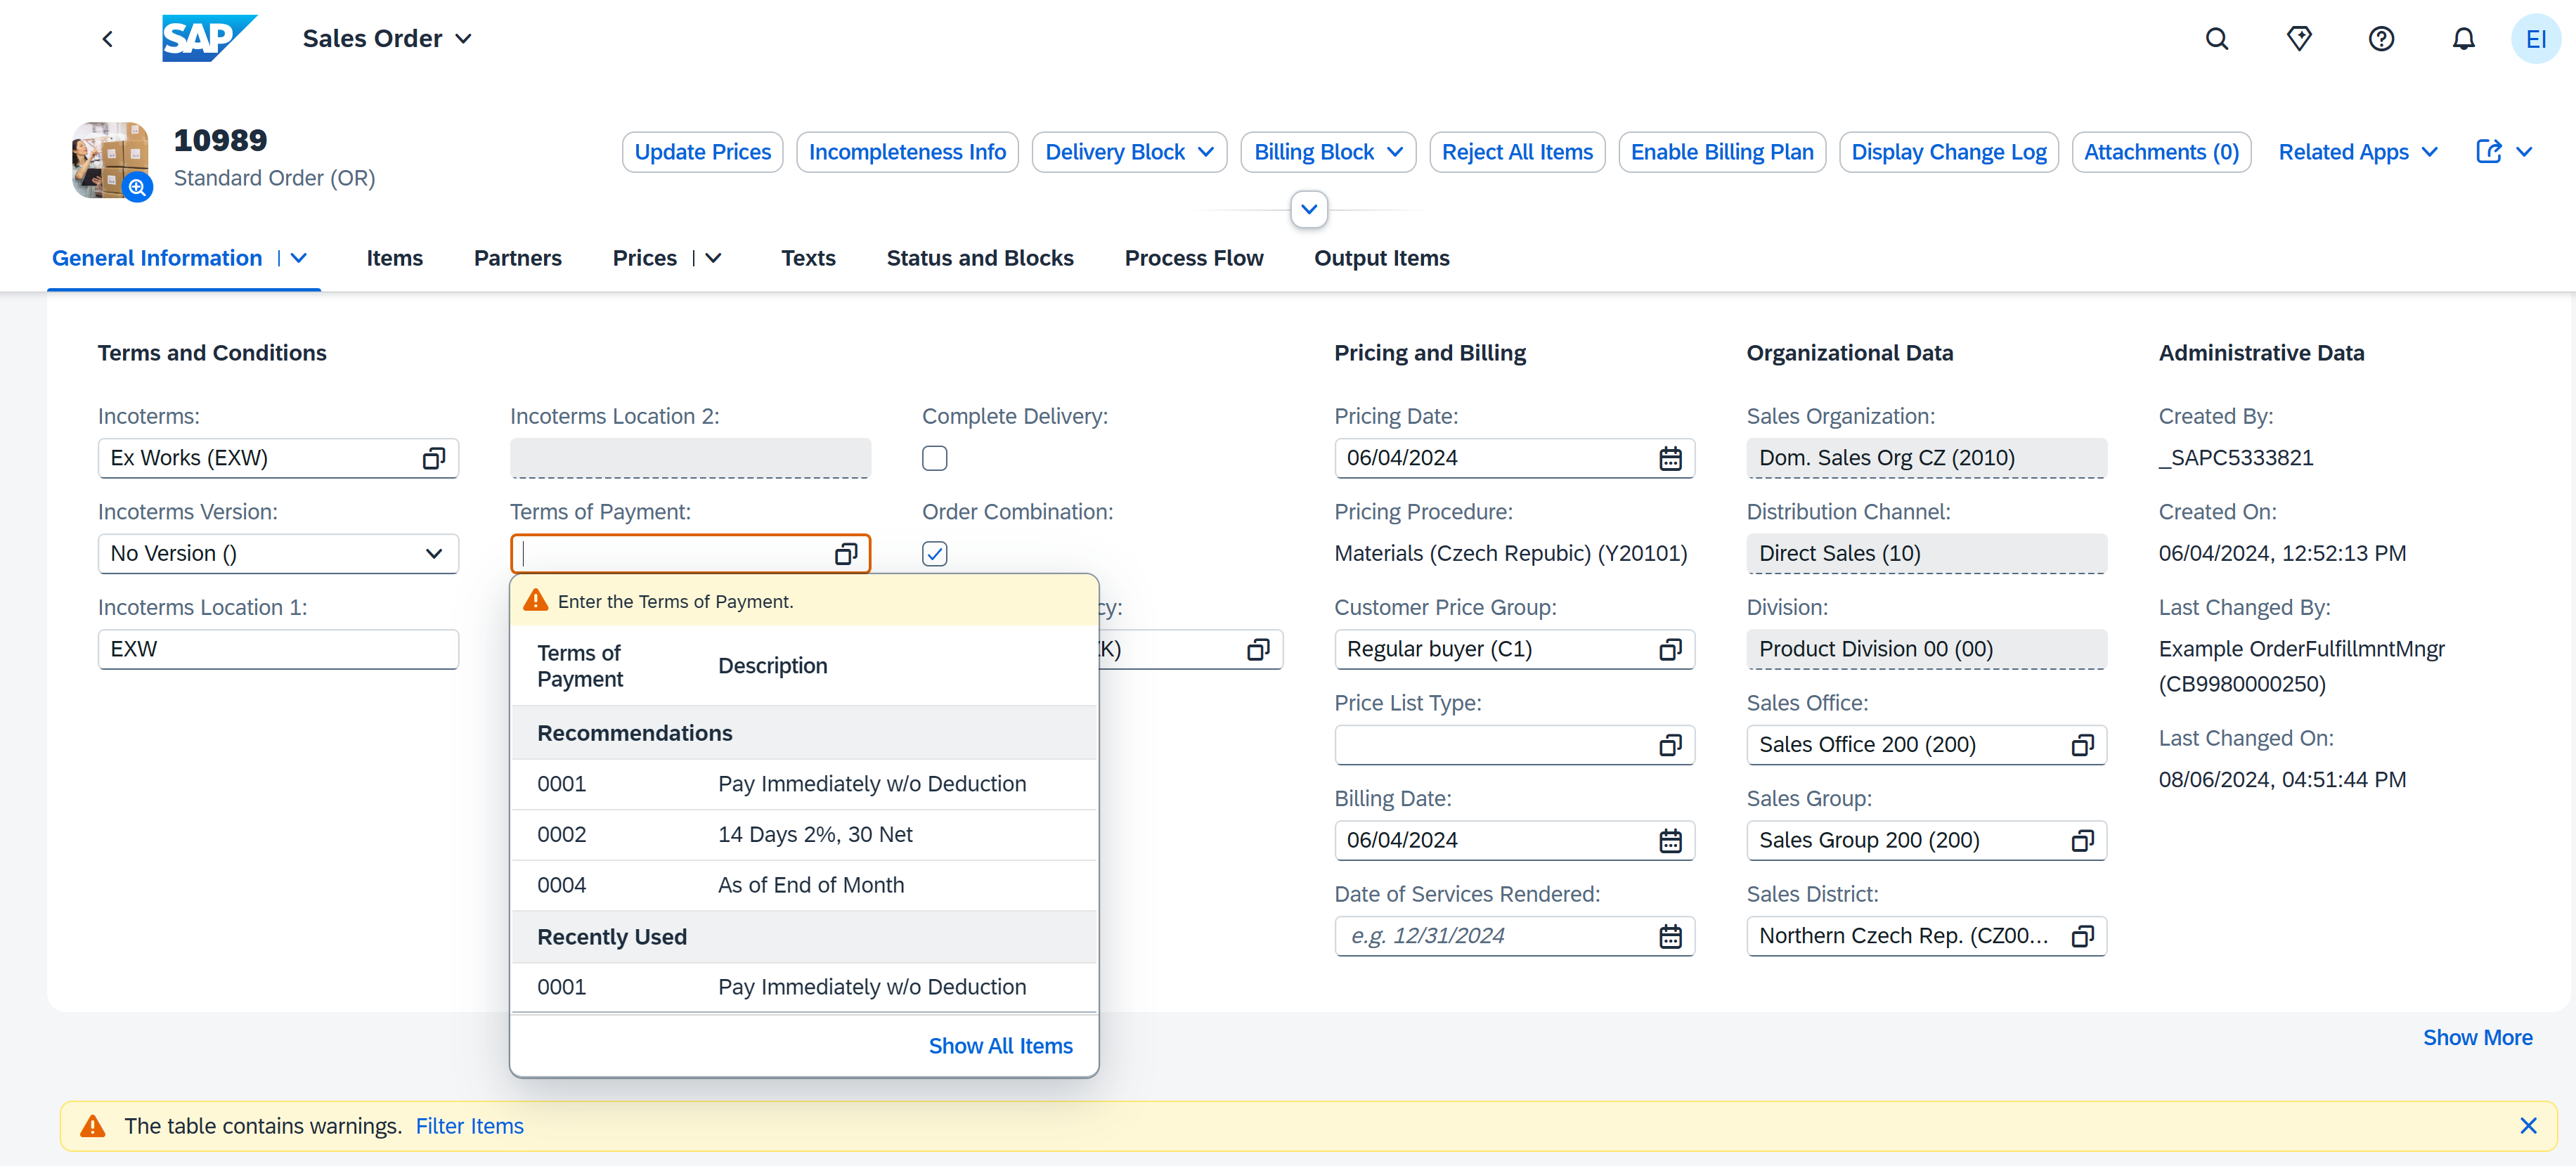
\includegraphics[width=0.8\linewidth]{figures/autocomplete_task.png}
    \caption{Illustrative example of a real-world autocomplete task, where the SAP S/4HANA Sales Order User interface \citep{sap-salt} predicts payment terms based on other filled-in response fields.}
    \label{fig:autocomplete-example}
\end{figure}


\subsection{List of predictive task descriptions}

\begin{enumerate}
  \item \texttt{rel-amazon}
    
    Autocomplete Regression:
    \begin{itemize}
      \item \texttt{review-rating}: For each review, predict the star rating.
    \end{itemize}


  \item \texttt{rel-arxiv}

  Forecasting Classification:
  \begin{itemize}
    \item \texttt{paper-citation}: For each paper, predict whether it will receive at least one citation in the next 6 months.
    \item \texttt{author-category}: For each author, predict the primary research category in which they will publish most in the next 6 months.
  \end{itemize}

  Forecasting Regression:
  \begin{itemize}
    \item \texttt{author-publication}: For each author, predict how many papers they will publish in the next 6 months.
  \end{itemize}

  Recommendation:
  \begin{itemize}
    \item \texttt{paper-paper-cocitation}: For each paper, predict which other papers will be co-cited with it in the next 6 months.
  \end{itemize}

  \item \texttt{rel-avito}

  Autocomplete Classification:
  \begin{itemize}
    \item \texttt{searchstream-click}: For each search session, predict whether the user clicked on a result.
    \item \texttt{searchinfo-isuserloggedon}: For each search, predict whether the user was logged in.
  \end{itemize}


  \item \texttt{rel-trial}

  Autocomplete Classification:
  \begin{itemize}
    \item \texttt{studies-has\_dmc}: For each study, predict whether it has a data monitoring committee.
    \item \texttt{eligibilities-adult}: For each study, predict whether it includes adult participants.
    \item \texttt{eligibilities-child}: For each study, predict whether it includes child participants.
  \end{itemize}

  Autocomplete Regression:
  \begin{itemize}
    \item \texttt{studies-enrollment}: For each study, predict the enrollment count.
  \end{itemize}


  \item \texttt{rel-event}

  Autocomplete Classification:
  \begin{itemize}
    \item \texttt{event\_interest-interested}: For each user--event interaction, predict whether the user marked the event as ``interested.''
    \item \texttt{event\_interest-not\_interested}: For each user--event interaction, predict whether the user marked the event as ``not interested.''
  \end{itemize}

  Autocomplete Regression:
  \begin{itemize}
    \item \texttt{users-birthyear}: For each user, predict the user's birth year.
  \end{itemize}


  \item \texttt{rel-f1}

  Autocomplete Regression:
  \begin{itemize}
    \item \texttt{results-position}: For each race result, predict the finishing position.
    \item \texttt{qualifying-position}: For each qualifying entry, predict the qualifying position.
  \end{itemize}

  Recommendation:
  \begin{itemize}
    \item \texttt{driver-circuit-compete}: Predict in which circuits a driver will compete in the next year.
  \end{itemize}

  \item \texttt{rel-hm} 

  Autocomplete Regression:
  \begin{itemize}
    \item \texttt{transactions-price}: For each transaction, predict the item price.
  \end{itemize}

  \item \texttt{rel-ratebeer} 

  Autocomplete Regression:
  \begin{itemize}
    \item \texttt{beer\_ratings-total\_score}: For each user, given a beer, predict the total score rating the user will give to the beer.
  \end{itemize}

  Forecasting Classification:
  \begin{itemize}
    \item \texttt{beer-churn}: For each beer, predict if it will receive zero ratings in the next 90 days.
    \item \texttt{user-churn}: For each active user, predict if they will rate zero beers in the next 90 days.
    \item \texttt{brewer-dormant}: For each brewer, predict if it will release zero beers in the next year (risk of going dormant).
  \end{itemize}

  Forecasting Regression:
  \begin{itemize}
    \item \texttt{user-count}: Predict the number of ratings a user will give in the next 90 days.
  \end{itemize}

  Recommendation:
  \begin{itemize}
    \item \texttt{user-beer-favorite}: For each user, predict the top 10 beers they will next add to their Favorites list.
    \item \texttt{user-beer-liked}: For each user, predict the top 10 beers they will rate at least 4.0 / 5.0.
    \item \texttt{user-place-liked}: For each user, predict the top 10 places they will rate at least 80 / 100.
  \end{itemize}

  \item \texttt{rel-salt}

  Autocomplete Classification:
  \begin{itemize}
    \item \texttt{item-plant}: For each sales order item, predict its plant (production/storage facility).
    \item \texttt{item-shippoint}: For each sales order item, predict its shipping point (dispatch location).
    \item \texttt{item-incoterms}: For each sales order item, predict its item-level international commercial terms.
    \item \texttt{sales-office}: For each sales order, predict the sales office responsible for managing sales activities for the relevant products and geographic region.
    \item \texttt{sales-group}: For each sales order, predict the sales group, i.e. the subdivision within the distribution chain that handles the customer and transaction.
    \item \texttt{sales-payterms}: For each sales order, predict the customer payment terms (payment deadlines/discounts).
    \item \texttt{sales-shipcond}: For each sales order, predict the shipping condition (logistics terms).
    \item \texttt{sales-incoterms}: Predict the header-level Incoterms (international commercial terms) for each sales order.
  \end{itemize}


  \item \texttt{rel-stack} 

  Autocomplete Classification:
  \begin{itemize}
    \item \texttt{badges-class}: For each badge, predict the badge class.
  \end{itemize}


  \item \texttt{rel-mimic} 

  Forecasting Classification:
  \begin{itemize}
    \item \texttt{patient-iculengthofstay}: For each patient admitted into the ICU, predict whether their stay will last at least 3 days.
  \end{itemize}

\end{enumerate}
